\documentclass[12pt,a4paper]{article}
\usepackage[utf8]{vietnam}
\usepackage{amsmath,amssymb}
\usepackage{tabularx}
\usepackage{tikz}
\usetikzlibrary{calc,angles,quotes,arrows.meta,patterns}
\usepackage{xcolor}
\usepackage{enumitem}
\usepackage{fancyhdr}
\usepackage[top=1.2cm, bottom=1.2cm, left=1.5cm, right=1.5cm]{geometry}
\usepackage[dethi]{ex_test}
\SAOPTN{widthSA=2.8,heightSA=0.62}

\setlength{\headheight}{15pt}
\setlength{\parskip}{0pt}

\pagestyle{fancy}
\fancyhf{}
\rhead{\textit{Môn Toán 6 -- Đề số 7}}
\lhead{\textit{Bộ đề ôn tập Giữa học kì I}}
\cfoot{\thepage}

\begin{document}

% --- KHUNG TIÊU ĐỀ ĐỀ THI ---
\noindent
\begin{tabularx}{\linewidth}{X r}
\textbf{TRƯỜNG THCS: \dotfill} & \textbf{ĐỀ KIỂM TRA ĐỊNH KỲ GIỮA HỌC KỲ I} \\
\textbf{Họ và tên: \dotfill} & \textbf{NĂM HỌC 2026 -- 2027} \\
\textbf{Lớp: \dotfill \quad SBD: \dotfill} & \textbf{Môn: TOÁN 6} \\
\hline
\end{tabularx}
\vspace{2mm}

\begin{center}
  \textbf{\large ĐỀ ÔN TẬP GIỮA HỌC KỲ I -- ĐỀ SỐ 7}\\
  \textit{Thời gian làm bài: 90 phút (Không kể thời gian phát đề)}
\end{center}
\vspace{1mm}

% --- PHẦN I ---
\noindent\textbf{\large PHẦN I. CÂU TRẮC NGHIỆM NHIỀU PHƯƠNG ÁN LỰA CHỌN (3,0 điểm)}

\textit{Thí sinh trả lời từ câu 1 đến câu 12. Mỗi câu hỏi thí sinh chỉ chọn một phương án duy nhất.}

\vspace{1mm}
\begin{ex}
Viết tập hợp các chữ số của số $2025$?
\choice
{$\{2; 0; 2; 5\}$}
{$\{2; 2; 5\}$}
{$\{2; 0; 2\}$}
{\True $\{0; 2; 5\}$}
\end{ex}

\begin{ex}
Hãy so sánh hai số tự nhiên $n = 52\,136\,001$ và $m = 52\,135\,998$:
\choice
{$n = m$}
{\True $n > m$}
{$n < m$}
{$n \le m$}
\end{ex}

\begin{ex}
Tính vận tốc của một ô tô biết rằng trong $6$ giờ ô tô đi được $324\text{ km}$:
\choice
{$48\text{ km/h}$}
{$51\text{ km/h}$}
{\True $54\text{ km/h}$}
{$57\text{ km/h}$}
\end{ex}

\begin{ex}
Cho hình bình hành có độ dài hai cạnh là $a, b$ và chiều cao tương ứng với cạnh đáy $a$ là $h$. Công thức tính diện tích của hình bình hành là:
\begin{center}
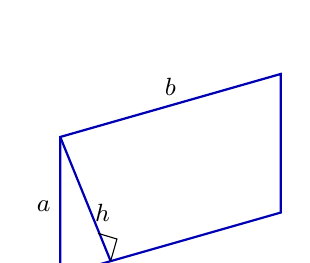
\begin{tikzpicture}[scale=0.8, font=\small]
  \coordinate (A) at (0,2.2);
  \coordinate (B) at (3.5,3.2);
  \coordinate (C) at (3.5,1);
  \coordinate (D) at (0,0);
  \draw[thick, blue!70!black] (A) -- (B) -- (C) -- (D) -- cycle;
  \draw[thick, blue!70!black] (A) -- (0.8,0.23) coordinate (H);
  \draw (0.8,0.23) -- (0.9,0.58) -- (0.6,0.67);
  \node[above] at (1.75,2.7) {$b$};
  \node[left] at (0,1.1) {$a$};
  \node[right] at (0.4,1) {$h$};
\end{tikzpicture}
\end{center}
\choice
{$S = a \cdot b$}
{$S = \dfrac{1}{2} a \cdot h$}
{$S = \dfrac{1}{2} b \cdot h$}
{\True $S = a \cdot h$}
\end{ex}

\begin{ex}
Bạn An có $125\,000$ đồng mang đến tiệm tạp hóa để mua bút gel, biết mỗi chiếc bút gel có giá $6\,900$ đồng. Hỏi bạn An có thể mua được nhiều nhất bao nhiêu chiếc bút gel?
\choice
{$0$ chiếc}
{\True $18$ chiếc}
{$19$ chiếc}
{$10$ chiếc}
\end{ex}

\begin{ex}
Hình nào sau đây có tất cả các cạnh bằng nhau?
\choice
{Tam giác đều, hình thoi, hình thang cân}
{Tam giác đều, hình bình hành, hình thang cân}
{\True Tam giác đều, hình thoi, hình vuông}
{Tam giác đều, hình bình hành, hình vuông}
\end{ex}

\begin{ex}
Cho hình bình hành $ABCD$. Hãy chọn khẳng định sai trong các khẳng định sau:
\begin{center}
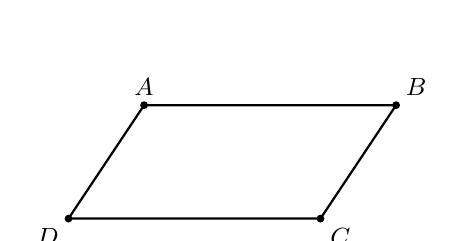
\begin{tikzpicture}[scale=0.8, font=\small]
  \coordinate (D) at (0,0);
  \coordinate (C) at (4,0);
  \coordinate (B) at (5.2,1.8);
  \coordinate (A) at (1.2,1.8);
  \draw[thick] (A) -- (B) -- (C) -- (D) -- cycle;
  \filldraw (A) circle (1.5pt) node[above] {$A$};
  \filldraw (B) circle (1.5pt) node[above right] {$B$};
  \filldraw (C) circle (1.5pt) node[below right] {$C$};
  \filldraw (D) circle (1.5pt) node[below left] {$D$};
\end{tikzpicture}
\end{center}
\choice
{$AB = CD, AD = BC$}
{$AB \parallel CD, AD \parallel BC$}
{\True $AB = BC = CD = DA$}
{Khẳng định A và B đều đúng}
\end{ex}

\begin{ex}
Cho $x$ là ước của $24$ và $10 \le x < 15$. Vậy $x$ có giá trị bằng:
\choice
{\True $12$}
{$13$}
{$14$}
{$10$}
\end{ex}

\begin{ex}
Biểu diễn tập hợp $H = \{1; 2; 3; 4; 5\}$ bằng cách chỉ ra tính chất đặc trưng của nó là:
\choice
{$H = \{x \in \mathbb{N} \mid x \le 5\}$}
{$H = \{x \in \mathbb{N} \mid x < 5\}$}
{\True $H = \{x \in \mathbb{N}^* \mid x \le 5\}$}
{$H = \{x \in \mathbb{N}^* \mid x < 5\}$}
\end{ex}

\begin{ex}
Trong các phân số sau, phân số nào là phân số tối giản?
\choice
{$\dfrac{26}{39}$}
{$\dfrac{15}{12}$}
{$\dfrac{27}{42}$}
{\True $\dfrac{3}{16}$}
\end{ex}

\begin{ex}
Số tự nhiên nào sau đây là ước của $12$?
\choice
{$0$}
{\True $4$}
{$5$}
{$10$}
\end{ex}

\begin{ex}
Nêu cách đọc chuẩn của số $123\,875$:
\choice
{\True Một trăm hai mươi ba nghìn tám trăm bảy mươi lăm}
{Một hai ba nghìn tám bảy năm}
{Một trăm hai ba tám trăm bảy năm}
{Một trăm hai mươi ba nghìn bảy trăm tám mươi lăm}
\end{ex}


\vspace{1mm}
\noindent\textbf{BẢNG TRẢ LỜI TRẮC NGHIỆM PHẦN I:}
\begin{center}
\begin{tabular}{|c|c|c|c|c|c|c|c|c|c|c|c|c|}
\hline
\textbf{Câu} & \textbf{1} & \textbf{2} & \textbf{3} & \textbf{4} & \textbf{5} & \textbf{6} & \textbf{7} & \textbf{8} & \textbf{9} & \textbf{10} & \textbf{11} & \textbf{12} \\
\hline
\textbf{Chọn} & \rule{0pt}{0.65cm} & & & & & & & & & & & \\
\hline
\end{tabular}
\end{center}
\vspace{2mm}

\setcounter{ex}{0}
\noindent\textbf{\large PHẦN II. CÂU TRẮC NGHIỆM ĐÚNG SAI (2,0 điểm)}

\textit{Thí sinh trả lời câu 1 và câu 2. Trong mỗi ý a), b), c), d) ở mỗi câu, thí sinh chọn đúng hoặc sai.}

\vspace{1mm}
\begin{ex}
Cho biểu thức $M = 2^3 \cdot 3 - 5$. Xét tính đúng/sai của các khẳng định sau:
\choiceTF
{Giá trị của lũy thừa $2^3$ là $6$}
{Khi tính giá trị biểu thức $M$, ta thực hiện phép nhân trước, phép trừ sau}
{\True Giá trị của biểu thức $M$ là $19$}
{\True Giá trị của biểu thức $M$ là một số nguyên tố}
\end{ex}

\begin{ex}
Cho hình chữ nhật $ABCD$ có chiều dài $AB = 8\text{ cm}$ và chiều rộng $BC = 6\text{ cm}$. Xét tính đúng/sai của các khẳng định sau:
\choiceTF
{Bốn cạnh của hình chữ nhật $ABCD$ có độ dài bằng nhau}
{\True Các cạnh đối diện $AB$ và $CD$ song song và bằng nhau}
{Hai đường chéo $AC$ và $BD$ vuông góc với nhau}
{\True Chu vi của hình chữ nhật $ABCD$ là $28\text{ cm}$}
\end{ex}


\noindent\textbf{BẢNG TRẢ LỜI PHẦN II:}
\begin{center}
\begin{tabular}{|c|c|c|c|c||c|c|c|c|c|}
\hline
\textbf{Câu 1} & \textbf{a)} & \textbf{b)} & \textbf{c)} & \textbf{d)} & \textbf{Câu 2} & \textbf{a)} & \textbf{b)} & \textbf{c)} & \textbf{d)} \\
\hline
\textbf{Đ/S} & \rule{0pt}{0.6cm} & & & & \textbf{Đ/S} & & & & \\
\hline
\end{tabular}
\end{center}
\vspace{2mm}

\setcounter{ex}{0}
\noindent\textbf{\large PHẦN III. CÂU HỎI TRẢ LỜI NGẮN (2,0 điểm)}

\textit{Thí sinh trả lời câu 1 và câu 2. Điền kết quả số vào ô trống tương ứng.}

\vspace{1mm}
\begin{ex}
Tìm các chữ số $x, y$ để số $\overline{35x98y}$ chia hết cho cả 2, 5 và 9. \shortans{x = 2, y = 0}
\end{ex}

\begin{ex}
Một hình thoi có độ dài hai đường chéo lần lượt là $8\text{ cm}$ và $10\text{ cm}$. Tính diện tích của hình thoi đó (theo đơn vị $\text{cm}^2$). \shortans{40}
\end{ex}


\setcounter{ex}{0}
\noindent\textbf{\large PHẦN IV. TỰ LUẬN (3,0 điểm)}

\textit{Thí sinh trình bày chi tiết lời giải vào giấy làm bài.}

\vspace{1mm}
\begin{ex} (1,0 điểm)
Thực hiện phép tính và tìm ước:
\begin{enumerate}[label=\textbf{\alph*)}, leftmargin=0.8cm, itemsep=2pt]
\item (0,5 điểm) Thực hiện phép tính: $6250 : \{50^2 : [112 - (32 - 2^2 \cdot 5)]\}$
\item (0,5 điểm) Tìm số tự nhiên $x \in Ư(30)$ thỏa mãn $x < 10$.
\end{enumerate}
\end{ex}
\vspace{1.5mm}

\begin{ex} (1,0 điểm)
Phân tích các số sau ra thừa số nguyên tố:
\begin{enumerate}[label=\textbf{\alph*)}, leftmargin=0.8cm, itemsep=2pt]
\item (0,5 điểm) $60$
\item (0,5 điểm) $125$
\end{enumerate}
\end{ex}
\vspace{1.5mm}

\begin{ex} (1,0 điểm)
Bài toán hình học thực tế:
\begin{enumerate}[label=\textbf{\alph*)}, leftmargin=0.8cm, itemsep=2pt]
\item (0,5 điểm) Nêu các bước vẽ tam giác đều có độ dài cạnh bằng $3\text{ cm}$.
\item (0,5 điểm) Tính chu vi và diện tích mảnh đất có hình vẽ dưới đây:
\begin{center}
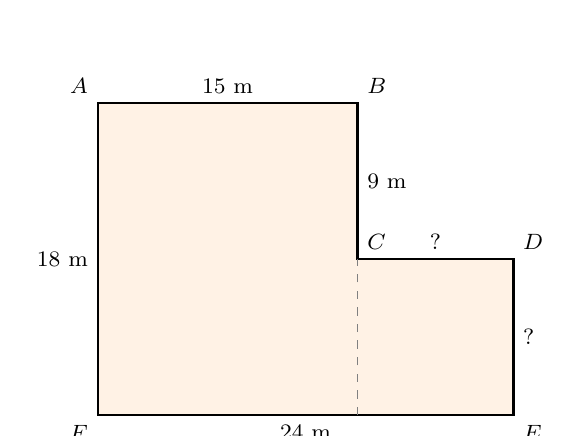
\begin{tikzpicture}[scale=0.22, font=\footnotesize]
  % Toa do cac dinh: A(0,18), B(15,18), C(15,9), D(24,9), E(24,0), F(0,0)
  \coordinate (F) at (0,0);
  \coordinate (A) at (0,18);
  \coordinate (B) at (15,18);
  \coordinate (C) at (15,9);
  \coordinate (D) at (24,9);
  \coordinate (E) at (24,0);
  \draw[thick, fill=orange!10] (A) -- (B) -- (C) -- (D) -- (E) -- (F) -- cycle;
  \draw[dashed, gray] (15,0) -- (15,9);
  \node[above] at (7.5,18) {$15\text{ m}$};
  \node[right] at (15,13.5) {$9\text{ m}$};
  \node[above] at (19.5,9) {$?$};
  \node[right] at (24,4.5) {$?$};
  \node[below] at (12,0) {$24\text{ m}$};
  \node[left] at (0,9) {$18\text{ m}$};
  \node[above left] at (A) {$A$};
  \node[above right] at (B) {$B$};
  \node[above right] at (C) {$C$};
  \node[above right] at (D) {$D$};
  \node[below right] at (E) {$E$};
  \node[below left] at (F) {$F$};
\end{tikzpicture}
\end{center}
\end{enumerate}
\end{ex}
\vspace{1.5mm}


\begin{center}
\rule{4cm}{0.4pt}\\
\textit{--- HẾT ---}
\end{center}
\end{document}
